\documentclass{standalone}
\usepackage{tikz}
\usetikzlibrary{shapes.geometric, arrows}

\tikzstyle{process} = [ellipse, minimum width=3cm, minimum height=1cm, text centered, draw=black]
\tikzstyle{arrow} = [thick,->,>=stealth]
\tikzstyle{box} = [rectangle, minimum width=3cm, minimum height=1cm, text centered, draw=black]

\begin{document}
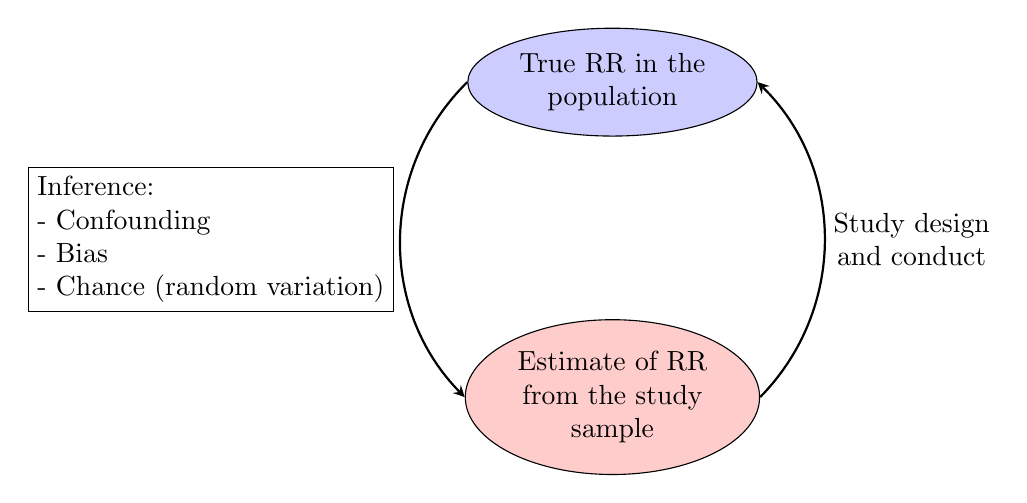
\begin{tikzpicture}[node distance=2cm]

% Nodes
\node (trueRR) [process, align=center, fill=blue!20] {True RR in the \\ population};
\node (estimateRR) [process, align=center, fill=red!20, below of=trueRR, yshift=-2cm] {Estimate of RR \\ from the study \\ sample};
\node (inference) [box, align=left, left of=trueRR, xshift=-3.1cm, yshift=-2cm] {Inference: \\ - Confounding \\ - Bias \\ - Chance (random variation)};
\node (studyDesign) [right of=trueRR, align=center, xshift=1.8cm, yshift=-2cm] {Study design \\ and conduct};

% Arrows
\draw [arrow] (trueRR.west) to [bend right=45] (estimateRR.west);
\draw [arrow] (estimateRR.east) to [bend right=45] (trueRR.east);

\end{tikzpicture}
\end{document}
